\documentclass[dvipdfmx,cjk,t,10pt]{beamer}  
%\documentclass[cjk,t]{beamer}


\usepackage{kasailab_slide_def}
\usepackage{color}
\usepackage{lastpage}
\setbeamertemplate{footline}[text line]{%
  \parbox{1.00\linewidth}{
    \vspace*{-8pt}\hspace*{-20pt}\textcolor{gray}{KASAI Laboratory, WASEDA University. All Rights Reserved.}}
  \hfill%
  \parbox{0.07\linewidth}{
    \vspace*{-8pt} \hfill \textcolor{gray}{\raggedright\insertpagenumber /{}\pageref{LastPage}}
  }
} 

%%目次スライド 
% 研究進捗では使用しないこと
%\AtBeginSection[]{
%    \frame{\tableofcontents[currentsection, hideallsubsections]} 
%}




\begin{document}



\title{○○○○○○手法の提案}

%\author{Hiroyuki }
\author[shortname]{氏名}
\institute[shortinst]{早稲田大学 基幹理工学部 \{情報通信学科,情報理工学科,情報理工・通信専攻\}}
%\date{2019年5月15日}

\begin{frame}
\titlepage
	\begin{center}	
	
\includegraphics[width=0.40\hsize]{waseda.eps}
	\end{center}	
	\vspace*{-0.5cm}
\end{frame}


\section{はじめに}

\begin{frame}
\frametitle{概要}
%\framesubtitle{sub title}

	\begin{screen}
		本スライド\IMPR{のみ}で研究(発表)の内容を説明できるような記述を心がけること.
	\end{screen}

	\begin{itemize}
	\item 本研究(本発表)の位置付け	の整理
	\itemspace	
	\item 具体的には
		\begin{itemize}
		\item 何を\IMPR{目的}として
		\item どのような\IMPR{技術課題}に対して
		\item どのような\IMPR{提案}(\IMPR{コア・アイデア}を提案)をし
		\item どのような(暫定的な)\IMPR{成果}(\IMPR{進捗})を得たのか?
		\end{itemize}
		について端的に分かるように記述する.
	\itemspace
	\item \underline{進捗報告の場合}:前回からの進捗
		\begin{itemize}
		\item 前回から本日まで\IMPR{何を進めてきたか?}
		\item 前回の発表との\IMPR{差分は何か?}
		\end{itemize}		
	\end{itemize}		
\end{frame}

\begin{frame}
\frametitle{研究背景および目的}
	\begin{itemize}
	\item 研究背景
	\item 研究目的	
	\end{itemize}			
\end{frame}

\begin{frame}
\frametitle{提案内容の概要}
	\begin{itemize}
	\item  具体的な技術動向・従来手法・検討(次頁以降で詳述する)
		\begin{itemize}
		\item 研究目的に対してどのような研究が進められているか?
		\item どのような技術が提案されているか?
		\item 従来技術・手法の分類など
		\end{itemize}			
	\item 技術課題
		\begin{itemize}
		\item 今回着目する\IMPR{具体的な技術課題}は何か?
		\end{itemize}			
	\item 提案内容
		\begin{itemize}
		\item 着目する技術課題に対して\IMPR{どのようにアプローチするのか?}
		\item \IMPR{コアとなるアイデアは何か?}
		\end{itemize}		
	\end{itemize}	
\end{frame}

\section{従来研究}

\begin{frame}
\frametitle{従来研究の動向}

	\begin{screen}
		%\begin{itemize}
		%\item 
		本スライドでは,次項以降で説明する従来研究について
		\begin{itemize}
			\item \IMPR{何故それらに着目するのか?}
			\item ページ・時間を割いて\IMPR{何故それらを紹介する必要があるのか?}
		\end{itemize}	
		が分かるような説明の記述が必要		
	\end{screen}
	
	
	\begin{itemize}
	\item 手法・アプローチの分類と,それぞれの利点・短点のまとめ
	\item 今回着目する研究と着目する理由
	\end{itemize}	
\end{frame}

\begin{frame}
\frametitle{従来研究(1/2)}
	\begin{screen}
		不用意に詳細情報に立ち入らず\IMPR{後述する提案手法を理解する上で必要となる説明}に集中すること.
	\end{screen}
	\begin{itemize}
	\item 文献情報	
		\begin{itemize}		
		\item 著者
		\item タイトル
		\item 出版情報(論文誌,会議,技術報告の区別と号・巻・ページ番号などの詳細情報)		
		\item 出版年
		\item URL
		\end{itemize}			
	\item 技術課題
	\item 提案概要
	\item 成果
	\end{itemize}	
\end{frame}

\begin{frame}
\frametitle{従来研究(2/2)}
	\begin{itemize}
	\item 文献情報
	\item 技術課題
	\item 提案概要
	\end{itemize}	
\end{frame}

\section{提案手法}

\begin{frame}
\frametitle{概要}

	\begin{screen}
		\begin{itemize}
		\item 提案手法のスライドの最初のページから手法の詳細やアルゴリズムを説明する学生が多い.
		\item 最初に提案手法の\IMPR{基本的な位置付け}や,\IMPR{コアとなるアイデア・アプローチ}を説明すること.
		\end{itemize}			
	\end{screen}

	\begin{itemize}
	\item 着目する技術課題
		\begin{itemize}
		\item 技術課題(詳細)について何が問題なのか?
		\end{itemize}
	\item 基本的考え方・アプローチ
		\begin{itemize}
		\item 着目する技術課題について\IMPR{どのように解決}しようとしているのか?
		\end{itemize}	
	\item 研究の立ち位置・目標
		\begin{itemize}
		\item アルゴリズムの確立,理論解析の確立,数値評価よる有効性の確認,ゴールは何か?
		\item \underline{進捗報告の場合}:論文紹介では何故その論文に着目するのか?
		\end{itemize}		
	\end{itemize}	
\end{frame}

\begin{frame}
\frametitle{提案手法の詳細(1/2)}
\framesubtitle{提案手法のスライドが多い場合にはサブタイトルを使用することを推奨}

	\begin{itemize}
	\item xxx
	\item xxx
	\[
		H(z) = \sum_{k=-\infty}^{\infty} h[k] z^{-k}.
	\]	
	\end{itemize}	
\end{frame}

\begin{frame}
\frametitle{提案手法の詳細(2/2)}

	\begin{itemize}
	\item xxx
	\end{itemize}	
\end{frame}


\begin{frame}
\frametitle{提案アルゴリズム}

\begin{center}

\end{center}

\end{frame}


\begin{frame}
\frametitle{提案アルゴリズムの解析}
	\begin{itemize}
	\item 時間・空間計算量・複雑度の解析
	\item 収束性,誤差,・・・解析
	\end{itemize}		
\end{frame}

\section{評価実験}

\begin{frame}
\frametitle{実験概要}

	\begin{screen}
		\begin{itemize}
		\item 実験のスライドの最初から,実験条件等の詳細を説明する学生が多い.
		\item 最初に\IMPR{実験の目的}つまり\IMPR{何を明らかにするのか?}を説明すること.
		\end{itemize}			
	\end{screen}
	
	\begin{itemize}
	\item 実験の位置付け
		\begin{itemize}
		\item 何を目的とした実験なのか?
		\item 何を示すための実験なのか?
		\end{itemize}	
	\item 想定される結果は?			
	\end{itemize}		
\end{frame}

\begin{frame}
\frametitle{実験方法}
	\begin{itemize}
	\item 実験条件
	\item 比較手法
	\item ハイパーパラメータ設定条件	
	\item データセット
	\item 評価指標・メトリック
	\end{itemize}	
	
\begin{center}
\IMPB{Dataset specifications}

{%\small
\begin{tabular}{l||c|c|c|c}
\hline
Dataset & $C$ & $V$ & $d_v$ & $n^v$ \\
\hline
\hline
UCI-digit & 10& 3 & $[216, 76, 64]$  & 1000 \\
\hline
Prokaryotic & 4& 3& $[393, 3, 438]$ & 100\\
\hline
3-sources & 6& 3& $[3560,3631,3068]$ & 66\\
\hline
\end{tabular}
}
\end{center}		
\end{frame}

\begin{frame}
\frametitle{実験結果1}
	\begin{itemize}
	\item 表の行・列の意味
	\item グラフの軸,軸の範囲,線・線種の意味
	\end{itemize}	
	
	\begin{figure}[htbp]
	\begin{center}	
	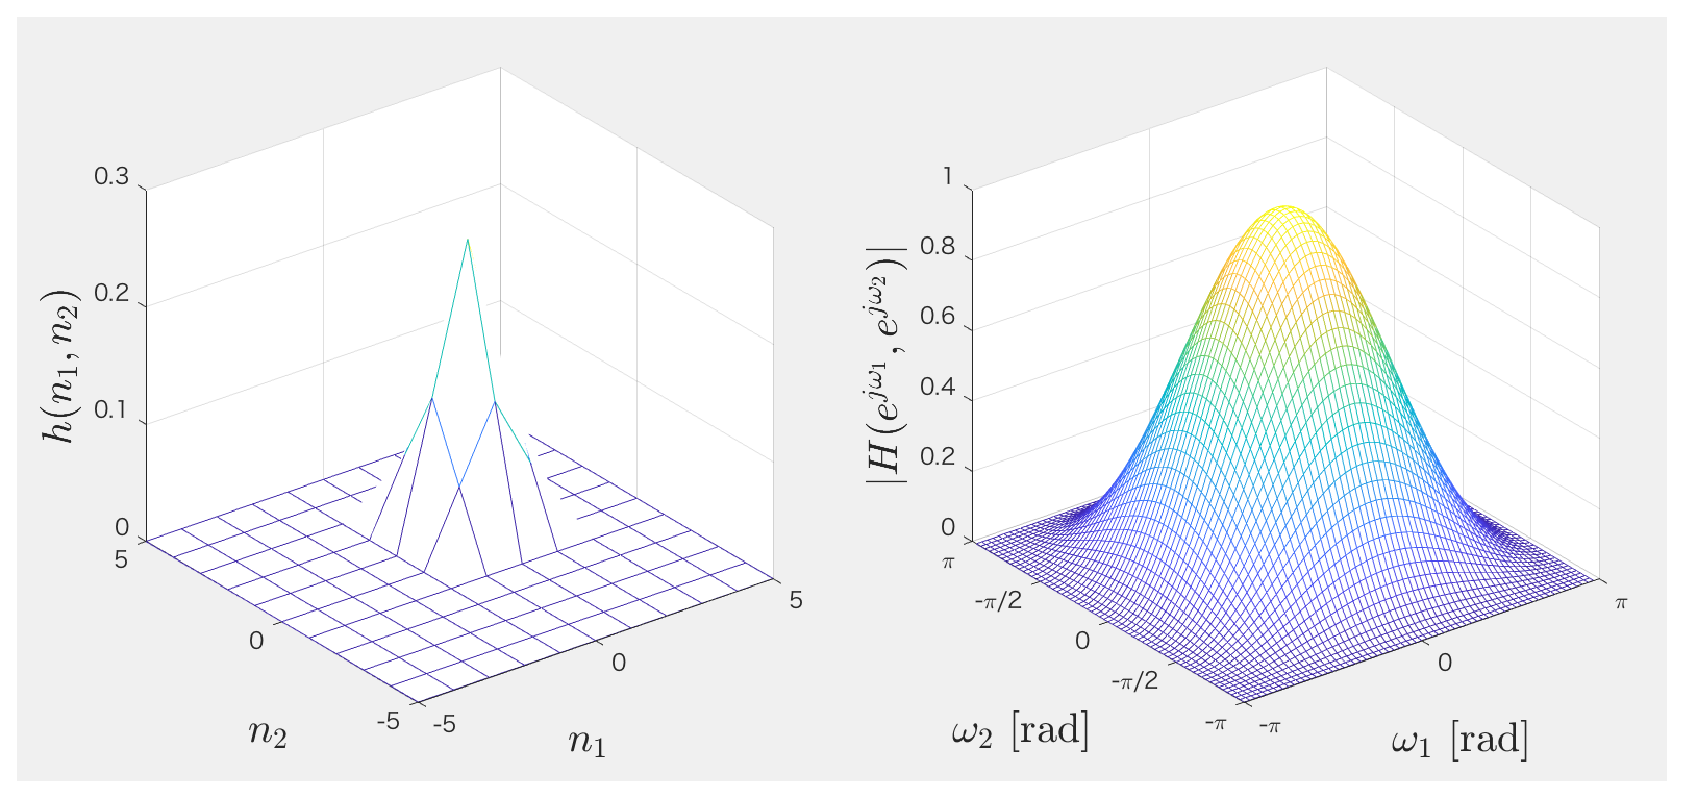
\includegraphics[width=0.85\hsize]{tmp.eps}
	\caption{Caption B.}
	\end{center}	
	\end{figure}				
\end{frame}

\begin{frame}
\frametitle{実験結果2}
	\begin{itemize}
	\item 表の行・列の意味
	\item グラフの軸,軸の範囲,線・線種の意味
	\end{itemize}		
	\vsp
	
	\begin{minipage}{0.46\hsize}
	\begin{figure}[htbp]
	\begin{center}	
	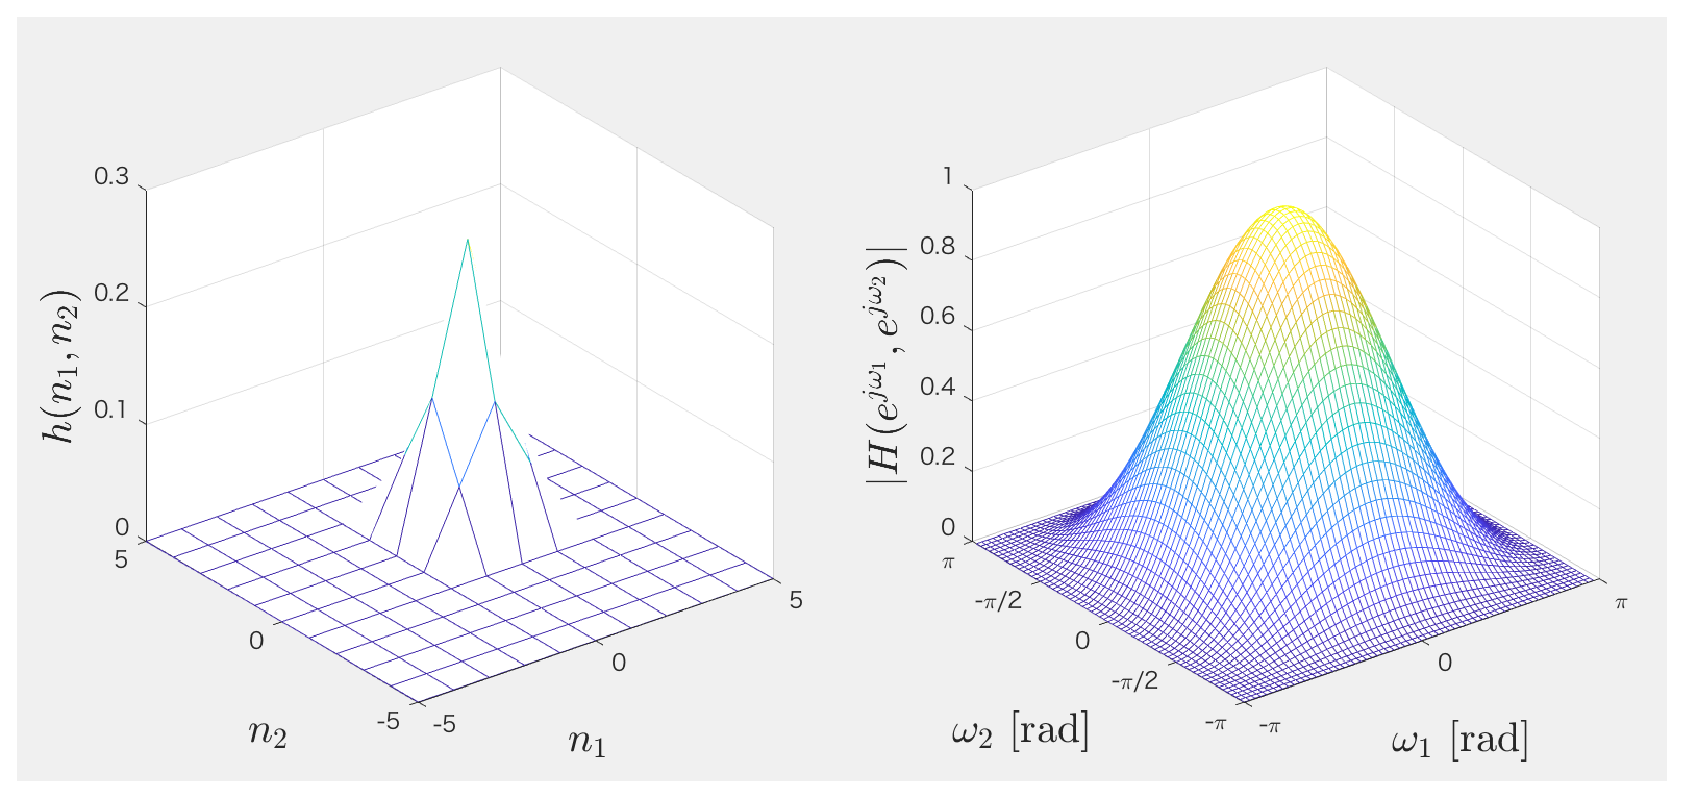
\includegraphics[width=0.95\hsize]{tmp.eps}
	\caption{Caption A.}

	\end{center}	
	\end{figure}	
	\end{minipage}
	\begin{minipage}{0.46\hsize}
	\begin{figure}[htbp]
	\begin{center}	
	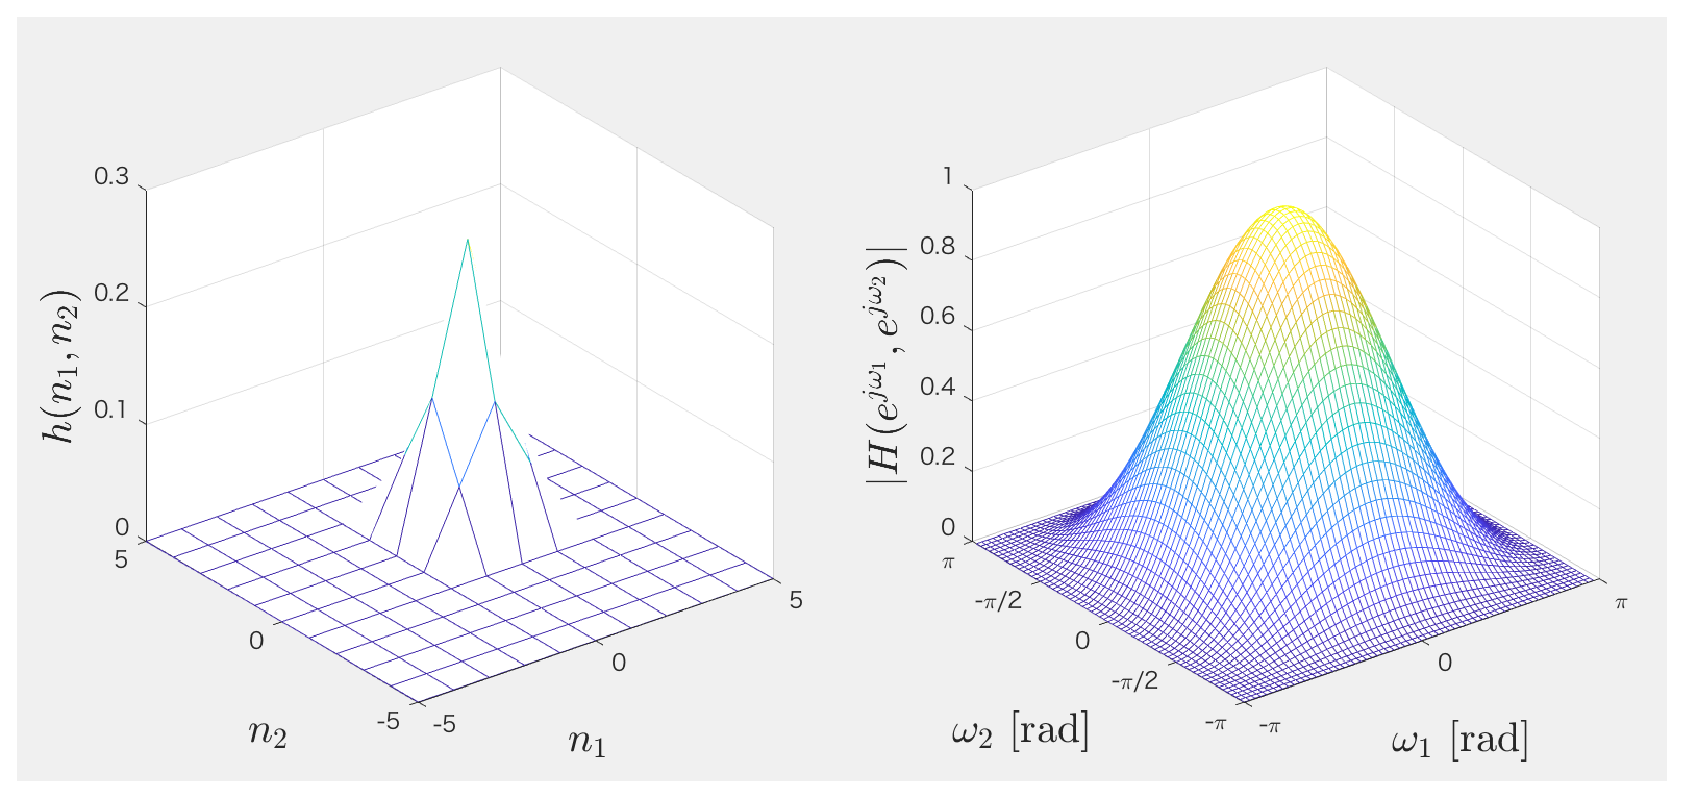
\includegraphics[width=0.95\hsize]{tmp.eps}
	\caption{Caption B.}
	\end{center}	
	\end{figure}		
	\end{minipage}		
\end{frame}

\begin{frame}
\frametitle{実験結果3}
\begin{center}
\IMPB{Averaged prediction error $(\%)$  with $1$-NN predictor (std) ($5$ trials).}
{\small
\begin{tabular}{l||c|c|c}
\hline
Methods & UCI-digit& Prokaryotic & 3-sources\\
\hline\hline
GMA \cite{Gillis_NN_2012} & 25.50 (1.72)& 42.62 (4.77) & 18.47 (4.89) \\
\hline
MFA  & 40.56 (9.20)& 42.26 (5.13) & 20.29 (6.29) \\
\hline
LPP  &24.82 (1.67) & 33.33 (4.56) & 18.41 (5.80) \\
\hline
MCCA & 32.80 (2.05) & 32.86 (2.82) & 29.12 (4.30)  \\
\hline
MvDA \cite{Lee_NIPS_2001}  & 27.84 (3.04)& 32.34 (4.96) & 21.95 (6.82) \\
\hline
L-MvMDA & 29.26 (2.84)& 38.20 (4.32) &15.93 (2.93) \\
\hline
S-LMvDA & 28.58 (2.25)& 36.85 (4.29) &16.17 (2.95) \\
\hline\hline
MvWDA-A & {17.31} (0.70)&  {31.40} (4.71) & \IMPB{\bf 15.69} (2.23) \\ 
\hline
MvWDA-B &\IMPB{\bf 17.22} (0.95) & \IMPR{\bf 24.20} (0.90) &\IMPR{\bf 15.04} (2.68) \\ 
\hline
MvWDA-C & 17.31 (0.90) & \IMPB{2\bf 4.38} (0.71) &17.58 (0.61) \\ 
\hline
MvWDA-D &\IMPR{\bf 16.99} (0.56) &29.82 (2.82)  &16.52 (2.81) \\ 
\hline
\end{tabular}
}
\end{center}
\end{frame}


\begin{frame}
\frametitle{実験考察}
	\begin{itemize}
	\item 実験結果から得られる内容の整理
	\item 想定していた結果との差異
	\item 実験結果から演繹される結論
	\item 不明な点
	\end{itemize}	
\end{frame}

\section{まとめと今後の課題}

\begin{frame}
\frametitle{まとめ}

	\begin{itemize}
	\item 提案の概要
	\item 実験の結果
	\item 成果・結論
	\end{itemize}	
\end{frame}

\begin{frame}
\frametitle{今後の課題}
	\begin{itemize}
	\item 残された課題は?
	\item 今後どのように研究を進めていくか?
		\begin{itemize}	
		\item 具体的な取り組み方法
		\item 新しい視点は?
		\item どのような実験を進めるのか?
		\end{itemize}	
	\item 今後のスケジュール
		\begin{itemize}	
		\item 研究作業スケジュール
		\item 学会投稿スケジュール
		\end{itemize}				
	\end{itemize}	
\end{frame}

\begin{frame}
\frametitle{\underline{進捗報告の場合}:今後の課題}
	\begin{itemize}
	\item 論文紹介の場合は,紹介した論文の内容から自身の研究にどのように結び付けていくか?について詳述する.
	\end{itemize}	
\end{frame}

\section{参考文献}

\begin{frame}[allowframebreaks]
%\setbeamertemplate{bibliography item}[text]
\setbeamertemplate{bibliography item}[triangle]
        \frametitle{References}
        %\bibliographystyle{amsalpha}
        \bibliographystyle{apalike}
        \bibliography{sample}
\end{frame}


\begin{frame}
	\begin{center}	
	\vspace*{1.0cm}
	\IMPB{\Large ご清聴ありがとうございました. }	
	
	\vsp\vsp
	\IMPB{\Large Thank you for listening. }
	\vspace*{1.0cm}
	
	
\includegraphics[width=0.50\hsize]{waseda.eps}
	\end{center}	
	\vspace*{-0.5cm}
\end{frame}

\begin{frame}
\begin{algorithm}[H]
\caption{Stochastic IBP algorithm}\label{alg:cap}
\begin{algorithmic}
\Procedure{SIBP}{$\pi,p$}
\Require Cost matrices  $C_1$,...$C_m$,probability measures $p_1$,...,$p_m$,$r>0$,
starting transport plans $\{\pi^{0}_{l}\}^{m}_{l=1}:\pi^{0}_{l}:=\exp(-\frac{C_l}{\gamma}),l=1,...,m,$ there exists $\hat{m}<<m$, and a subset $S$ of \{1,2,...,$m$\}, and $\|S\|=\hat{m}$
\Repeat
\If{t mod 2 = 0}
\State random sampling $S$
    \State $\boldsymbol{\pi}^{t+1}:=\underset{\boldsymbol{\pi} \in \mathcal{C}_{1}}{\operatorname{argmin}} \sum_{l=1}^{\hat{m}} w_{S_l} K L\left(\pi_{S_{l}} \mid \pi_{S_{l}}^{t}\right)$

\Else{}
    \State$ \boldsymbol{\pi}^{t+1}:=\underset{\pi \in \mathcal{C}_{2}}{\operatorname{argmin}} \sum_{l=1}^{\hat{m}} w_{S_l} K L\left(\pi_{S_l} \mid \pi_{S_l}^{t}\right)$ 
\EndIf
\State $t:= t+1$
\Until{Converge}
\EndProcedure

\end{algorithmic}
\end{algorithm}
\end{frame}
\end{document}





